
\textbf{Sensores}

Ao se expor todos os parâmetros de qualidade da água, é necessário se ter o conhecimento dos sensores que farão a
obtenção dessas informações. A seguir, se encontram uma série de sensores que foram pesquisados a fim de se ter uma 
idéia geral de quais equipamentos poderão ser utilizados no projeto. 

Sensores são dispositivos eletroeletrônicos que tem a propriedade de transformar em sinal elétrico a transformação
de uma grandeza física que esta relacionada a uma ou mais propriedade do material de que é feito o sensor. Esses elementos
são capazes de monitorar a variação de uma grandeza física e transmitir esta informação a um sistema em que a indicação
seja inteligível para nós ou para o elemento de controle do sistema. Os sensores são compostos por elementos denominados
transdutores que convertem uma grandeza de entrada em uma grandeza elétrica, que pode ser processada por um circuito
elétrico ou eletrônico \cite{vinay00}.

Existem diversos tipos de sensores os que julgamos necessários para o controle do sistema de capitação de água pela rotação
da turbina. São os sensores de umidade relativa do ar, sensores de velocidade e direção do vento (anemômetro), sensores
de nível e fluxo de entrada e saída de água, sensores de oxigênio, sensores de condutividade, sensores de pH, sensores
de turbidez, sensores de nitrato/nitrogênio, entre outros.

  \begin{enumerate}
  
    \item \textbf{Sensor da umidade do ar e temperatura}
      
	Características:
	
	\begin{itemize}
	 \item Processamento digital de sinal
	 \item Umidade relativa e temperatura do ar em um único sensor
	 \item Alta acurácia de leitura e linearização
	 \item Sinais de saída condicionados
	 \item Excelente estabilidade de longo termo
	 \item Baixo tempo de resposta
	 \item 100\% intercambialidade
	\end{itemize}

	Construção:
	
	O invólucro do sensor e do circuito eletrônico é moldado em plástico injetado e estabilizado para U.V.
	O invólucro do circuito é selado, sendo à prova de respingos e poeira. Todas as conexões elétricas
	são feitas através de um conector selado na base do sensor. O sensor opera de 0 a 100\% umidade relativa.
	Os transdutores internos não sofrem danos mesmo com condensação. O circuito digital do sensor realiza a
	compensação de temperatura e a linearização do sinal de saída. O armazenamento dos dados de calibração do
	 sensor em memória interna não volátil fornece uma maior acurácia nas leituras.
	 
	 \begin{figure}[!htbp]
	  \centering
	  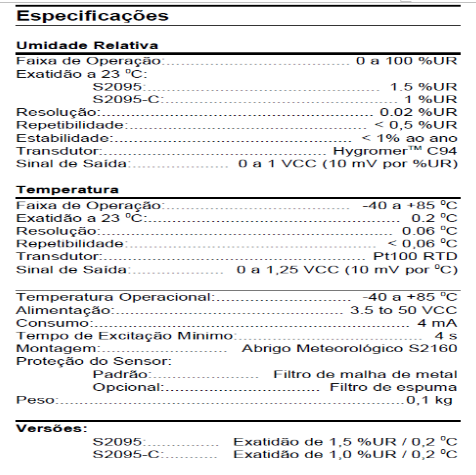
\includegraphics[scale=0.5]{editaveis/figuras/especificacao_sensor_umidade}
	  \caption[Especificação do sensor de umidade e temperatura]{Especificação do sensor de umidade e temperatura. \footnotemark}
	  \FloatBarrier
	  \label{especificacao_sensor_umidade}
	 \end{figure}
	 \footnotetext{Fonte: \cite{squitter}}
	 
    \item \textbf{Sensor de pH}
    
	O sensor de pH da água é de extrema importância para o projeto da “planta de abastecimento de água potável
	através da umidade do ar” pois monitora um dos índices de qualidade da água especificados pela \cite{anaGov}.
	
	\begin{center}
	 \textbf{Especificação do sensor de pH}
	\end{center}

	Para aplicações industriais, o método de medição de pH mais empregado é o eletrodo de vidro \cite{sole79}.
	Os eletrodos de pH possuem basicamente o mesmo funcionamento que as baterias: transferem uma tensão mínima que poderá
	ser detectada por um medidor ou um regulador de pH. A diferença é que os eletrodos de pH não produzem tensão de forma
	contínua, a não ser quando são introduzidos num líquido.
	
	\begin{center}
	 \textbf{Calibração de sensores de pH}
	\end{center}
	
	O período de calibração de um sensor de pH depende do contexto em que o sensor será aplicado e do tipo de sensor
	que será utilizado. O tipo de sensor a ser utilizado pode variar de acordo com parâmetros como temperatura.
	O sensor de pH pode vir acoplado a um sensor de condutividade, entre outros. Apesar de existirem vários tipos,
	todo eletrodo de pH requer calibração periódica. Uma calibração em dois pontos caracteriza um eletrodo com um
	medidor de pH específico. Uma desvantagem dos sensores de pH é que eles necessitam de calibração diária.
	Neste caso, seria necessário um funcionário que realizasse a calibração diariamente, ou de um sistema automatizado
	que realize a calibração.
	
	
    \item \textbf{Sensor ORP}
    
	O sensor ORP é similar ao sensor pH quanto ao seu funcionamento, porém, ao invés de seu eletrodo ser envolvido por
	vidro, é geralmente envolvido por platina ou ouro, devido ao fato de esses metais não interferirem nas reações químicas.
	Nos sensores ORP, o gel interno recebe a corrente elétrica provinda do meio e a transmite ao interior do sensor.
	Posteriormente, o fio e prata pura transmite a corrente positiva ao para o cabo de conexão, que leva o sinal recebido
	ao controlador.
	
    \item \textbf{Sensor de turbidez}
    
	Os sensores de turbidez são necessários para aferir a quantidade de sólidos que existem na água, já que este é um dos
	índices de qualidade da água definidos pela ANA.
	
	\begin{center}
	 \textbf{Especificação do sensor de turbidez}
	\end{center}
	
	O sensor de turbidez é o equipamento utilizado para medir a turbidez de um líquido. A aferição compara o espalhamento
	de um feixe de luz ao passar pela amostra, com o de um feixe de igual intensidade, ao passar por uma suspensão
	padrão \cite{usepa99}. Os sensores de turbidez funcionam por meio de detectores fotoelétricos, que são sensíveis
	a sutis mudanças na intensidade da luz, proporcionando uma maior precisão. O sensor de turbidez utilizado
	atualmente é o turbidímetro nefelométrico. 
	
	\begin{center}
	 \textbf{Funcionamento do sensor de turbidez}
	\end{center}
	
	O princípio de funcionamento dos turbidímetros atuais, baseia-se na emissão de um feixe luminoso e na detecção da luz
	refletida pelas partículas em suspensão ou diferença de intensidade entre a luz emitida e recebida, a qual é convertida
	em sinal elétrico e mostrada no equipamento. Nos instrumentos comerciais o detector é disposto em ângulos de
	45, 90 ou 180 graus. A emissão de luz normalmente é obtida por meio de lâmpadas de mercúrio,lâmpadas de tungstênio,
	laser ou diodos de emissão \cite{padua06}. Os sensores de turbidez processam as informações analógicas 
	e as devolvem em forma de tensão.
	
	\begin{center}
	 \textbf{Calibração do sensor de turbidez}
	\end{center}
	
	A calibração do sensor de turbidez pode ser feita de três formas:
	
	\textbf{Calibração direta} na qual é utilizada uma solução padrão de formazina para a calibração do sensor.
	\textbf{Calibração Indireta} na qual a grandeza que deseja ser medida é fornecida por um meio externo, como um equipamento
	  previamente calibrado, que atua simultaneamente no Sistema de Medição em Calibração e no Sistema de Medição Padrão,
	  e é feita uma comparação com os resultados obtidos \cite{cni01}.
	\textbf{Via Software} na qual a calibração é feita por um software que pode ser realizada no próprio aparelho ou com a
	  utilização de um computador que faz a calibração quando o sensor é conectado. 
	
    \item \textbf{Sensor de temperatura da água}
	
	Os sensores de temperatura da água medem a temperatura da água e funcionam segundo o princípio de resistência variável.
	Os sensores de temperatura de líquidos em geral são envolvidos por materiais com alta resistência a corrosão.
	Estes sensores funcionam com transdutores, que são componentes que possuem a função de transformar grandezas elétricas.
	Basicamente, um sensor de temperatura é uma espécie de resistor que aumenta sua resistência quando a temperatura do
	líquido aumenta.
	
	\begin{center}
	 \textbf{Calibração do sensor de temperatura da água}
	\end{center}
	
	Uma das vantagens dos sensores de temperatura é o fato de que estes componentes não necessitam de calibração constante.
	Um dos métodos de calibração mais utilizados atualmente é o Método Comparativo no qual o sensor a calibrar tem sua
	indicação comparada com as de um padrão de referência. O método consiste em imergir ambos em um meio térmico uniforme
	e estável, cuja temperatura possa ser controlada na faixa requerida.
	
    \item \textbf{Anêmometro ultrasônico}
    
	Anemômetro é um equipamento que mede a velocidade e a direção dos ventos. No SI (Sistema internacional) a unidade
	utilizada para medir a velocidade do vento pode ser em m/s (metros por segundo), em km/h (quilômetros por hora) ou
	em nós \cite{almeida04}.
	
	No mercado existem vários tipos de anemômetros com diferentes exatidões, custo e métodos de medição, são alguns deles: 
	anemômetro de copo, termoelétrico e o ultrassônico.
	
	O anemômetro de copo é o mais utilizado e o mais comum no mercado \cite{cyliax06}. Ele possui vários copos ocos
	fixos em dois eixos, que se movem proporcionalmente com a velocidade do vento, que é indicada por um tacômetro. Este
	anemômetro é de baixo custo e possui precisão de mais ou menos 2\%, mas precisa ser calibrado e passar por manutenção
	periodicamente, pois tem partes móveis que se desgastam com o tempo e alteram a sua precisão.
	
	O anemômetro termoelétrico possui dois tipos o de fio e o de tubo, genericamente os dois tipos utilizam o calor dissipado
	pelos sensores do anemômetro para a medição da velocidade do vento, ou seja, o sensor é aquecido e o calor que é dissipado
	é proporcional a velocidade do vento.  O tempo de resposta do termoelétrico é maior do que o de copo, é não possui partes
	moveis, porém não é indicado para locais abertos, pois seus sensores são frágeis e os fios ou tubos acumulam impurezas,
	desse modo diminuindo sua precisão.
	
	O anemômetro ultrassônico é um tipo anemômetro que possibilita a medição da velocidade do vento , por meio da velocidade
	do som no ar.Possuisensores ultrassônicos dispostos em formato de tetraedro e em cada extremidade possui um sensor
	piezolétricos \cite{ribeiro06}, este sensor é um tipo de transdutor ultrassônicos que pode se comportar tanto
	como transdutor-transmissor quanto um transdutor-receptor, ou seja, ele pode gerar ondas ultrassônicas e também de
	recebê-las (KOYAMA,2007).
	
	O tempo que o pulso enviado por um dos sensores leva para chegar a um dos outros é medido e incrementado ou decrementado,
	dependendo da direção da velocidade do som, assim podendo obter-se a velocidade do vento nas três direções.
	
	\begin{figure}[!h]
	  \centering
	  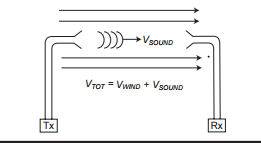
\includegraphics[scale=0.8]{editaveis/figuras/sinal_ultrasonico}
	  \caption[Soma do sinal ultrassônico e a velocidade do vento]
	    {Figura ilustrativa da soma do sinal ultrassônico e a velocidade do vento \cite{cyliax06}.}
	  \FloatBarrier
	  \label{sinal_ultrasonico}
	\end{figure}
	
	Este anemômetro é um dos mais confiáveis, não possui partes móveis, tem uma resposta rápida e com boa exatidão, não
	precisa de manutenção periódica epode ser utilizado em qualquer ambiente, sem comprometer sua precisão.
	
	Abaixo uma tabela de especificações técnicas de um anemômetro ultrassônico (Vaisala WINDCAP\textregistered WMT700):
	
	\begin{figure}[!h]
	  \centering
	  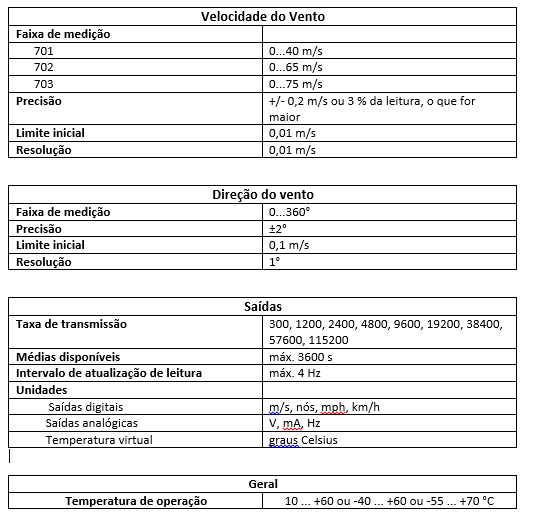
\includegraphics[scale=0.6]{editaveis/figuras/vaisala_spec}
	  \caption[Especificações técnicas do anemômetro ultrassônico Vaisala WINDCAP\textregistered WMT700]
	    {Especificações técnicas do anemômetro ultrassônico Vaisala WINDCAP\textregistered WMT700}
	  \FloatBarrier
	  \label{vaisala_spec}
	\end{figure}
    
    \item \textbf{Microcontroladores}
	
	O microcontrolador é uma espécie de computador que é programado para realizar funções de acordo com o que se deseja.
	Dentro de um computador de mesa (desktop), por exemplo, existem vários microcontroladores de vários modelos e tamanhos
	que realizam diversas funções diferentes. Ou seja, são dispositivos que geralmente são embutidos no interior de um produto
	que podem controlar as funções ou ações desse produto \footnotemark. 
	\footnotetext{Disponível em: <http://tecnologia.hsw.uol.com.br/microcontroladores1.htm>}
	
	No contexto em que se encaixa este documento, os microcontroladores serão responsáveis por fazerem leituras de sinais 
	que posteriormente poderão nos informar a qualidade da água, potência em que se está sendo trabalhada a turbina,
	quantidade de água armazenada no reservatório em tempo real, a velocidade atual em que o vento atinge as turbinas,
	umidade do ar, etc. Mas para a obtenção dessas diversas informações, é necessária a utilização dos vários sensores
	citados anteriormente que vão trabalhar de modo conjunto com os microcontroladores, que formam um sistema para ler
	essas informações.
	
	Inicialmente, ao se receber a informação dentro do sistema, ela tem de ser condicionada. O condicionador mais comum é
	o amplificador. Este tem a função de amplificar sinais de baixa intensidade a fim de se aumentar sua resolução. Logo
	após isto, este sinal é enviado a um filtrador que tem por função melhorar a freqüência enviada, ou seja, ele vai
	remover sinais indesejados fazendo a freqüência permanecer no formato desejado. Dependendo de cada sinal, deverá ser
	usado um filtro diferente, pois sinais AC e DC requerem tratamentos diferenciados. Por exemplo, sensores de temperatura 
	recolhem sinais DC que geralmente são de alta freqüência, com isto, os filtradores buscam deixar esse sinal mais tênue.
	Posteriormente também se pode amplificar novamente o sinal. Essa etapa geralmente depende da ordem em que a tensão está
	chegando. Uma tensão da ordem de micro volts pode requerer ser amplificada mais uma vez para que seja sensível ao
	microcontrolador. Em sequência, o sinal deve passar por um conversor analógico digital, que tem por função passar
	informação do nosso mundo, como luz, som, para o formato digital, e então é enviado para um microcontrolador. A partir
	dessa etapa, o microcontrolador passa a informação para um transmissor que envia a informação para uma central \footnotemark.
	
	\footnotetext{Disponível em: <http://www.sabereletronica.com.br/artigos/2805-condicionamento-de-sinais-analgicos-e-sensores>}
	
	A figura ~\ref{funcionamento_microcontrolador} ilustra o funcionamento desse sistema.
	
	\begin{figure}[!h]
	  \centering
	  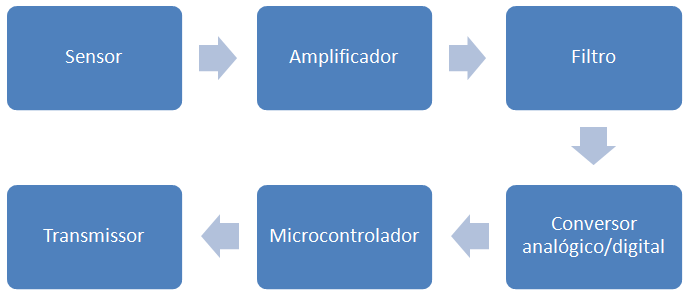
\includegraphics[scale=0.6]{editaveis/figuras/funcionamento_microcontrolador}
	  \caption[Processamento do sinal]{Processamento do sinal}
	  \FloatBarrier
	  \label{funcionamento_microcontrolador}
	\end{figure}
	
  \end{enumerate}
  
  \vfill